\section{What a page type owns on disk}
\label{sec:page-types}

A board page type has always been described by what a page \emph{is}: how it
resolves, how it closes, which typed records it fills. That description is
complete for reading a page and incomplete for building one, because a page of
some types also owns files. Ten contracts govern the types today and between
them they name six artifact paths, so a writer opening a display page for the
first time learns what the page must argue and not what folders it must create.

Five shapes cover the ten types. A \textsc{unit} type owns a folder on both
sides, an authoring folder that is worked in and a shipped folder that is
generated from it; display and slide are its two members. A \textsc{section}
type owns one flat file at the paper root and never a subdirectory of its own.
A \textsc{qa-probe} type owns a folder of evidence records named for the page
that asked; literature and value are its two members, and literature also emits
a bibliography generated from a shared bank. A \textsc{mirror} type owns nothing
and annotates a folder someone else already maintains: venue points at a shared
venue playbook, design at the candidate folder its downstream display unit keeps,
and skill at the skill folder it mirrors. A \textsc{none} type owns nothing at
all, which is the honest answer for stage and meeting.

The shapes are not symmetric in who may act on them, and the display unit shows
this most sharply. Figure~\ref{fig:display-pipeline} draws the eleven steps that
produce one unit. Two of the eleven may be taken by a script, and both are
mechanical: compiling the standalone preview, and copying the selected artifact
into the shipped tree. The rest are a person's, and the three steps of the
acceptance lane are a person's without exception. A machine may render a display
and may ship it. No machine may accept one, because acceptance is of a specific
render rather than of a name, and only a reader can say that the thing in front
of them carries the claim it was asked to carry.

%% GENERATED by board/haipipe-board/cli/build-displays.py from
%%   ../display/QBt3-for-display/float.tex
%% Do not edit this file. Edit the copy under ../display/ and rebuild.
\begin{figure}[t]
  \centering
  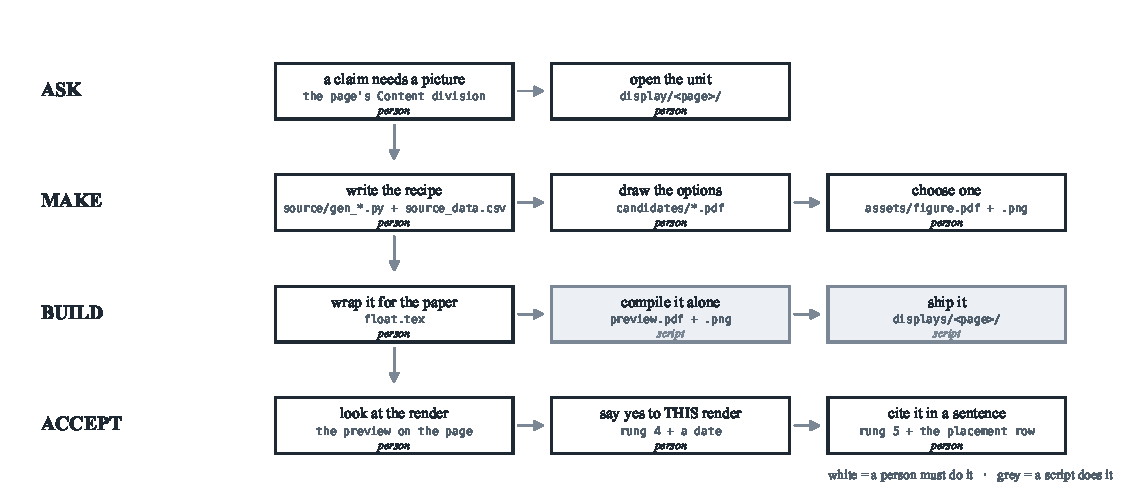
\includegraphics[width=0.95\textwidth]{displays/QBt3-for-display/assets/figure.pdf}
  \caption{How one display unit is produced, and who is allowed to do each step.
  Four lanes, eleven steps, read left to right within a lane and top to bottom
  between them. A white box is a step a person must take; a grey box is a step a
  script takes. Only two of the eleven are grey, and both sit in BUILD: the
  standalone preview compile, and the copy into \texttt{displays/}. Every step in
  ACCEPT is white, which is the rule this figure exists to make visible: a
  machine may render a display and may ship it, and no machine may accept one.
  Drawn from \texttt{source/source\_data.csv} at build time; the lane order is
  the only thing the plotting code hardcodes.}
  \label{fig:display-pipeline}
\end{figure}


The practical consequence is that a contract stated in prose cannot fail, and a
specimen can. A prose contract that never mentions \texttt{float.tex} reads
exactly as well as one that does; a specimen folder missing \texttt{float.tex}
does not build. That asymmetry is the argument for keeping a worked example of
every type on disk and running the real tooling against it, rather than
describing each type and trusting the description.
